
\documentclass[11pt,a4paper]{article}
\usepackage[margin=2.2cm]{geometry}
\usepackage{amsmath,amssymb,graphicx,booktabs}
\usepackage{caption,float,enumitem}
\usepackage[T1]{fontenc}
\usepackage[hidelinks]{hyperref}

\captionsetup{font=small,labelfont=bf}
\setlist{itemsep=2pt,topsep=4pt}
\newcommand{\code}[1]{\texttt{\small #1}}

\title{Assignment 1: Multi-Instance Object Recognition in Cluttered Scenes}
\author{}
\date{}

\begin{document}
\maketitle
\vspace{-0.8cm}

\section{Objective}

The goal of this assignment is to detect and localise multiple instances of a
known object in a single cluttered photograph. Instances may differ in scale
and orientation and may be partly occluded by other objects. The pipeline uses
OpenCV for image I/O and SIFT feature extraction. Feature matching,
parameter-space clustering, geometric estimation, verification and duplicate
suppression are implemented in the accompanying code.

\section{Data}

\begin{itemize}
  \item \textbf{Template.} An isolated photograph of a Kurkure packet
        (\code{data/template.png}, 2591$\times$3674).
  \item \textbf{Query scene.} A photograph of my lab desk
        (\code{data/scene.png}, 4032$\times$3024) containing several
        Kurkure packets among other clutter, at different distances and
        orientations, with partial occlusion.
\end{itemize}

\begin{figure}[H]\centering
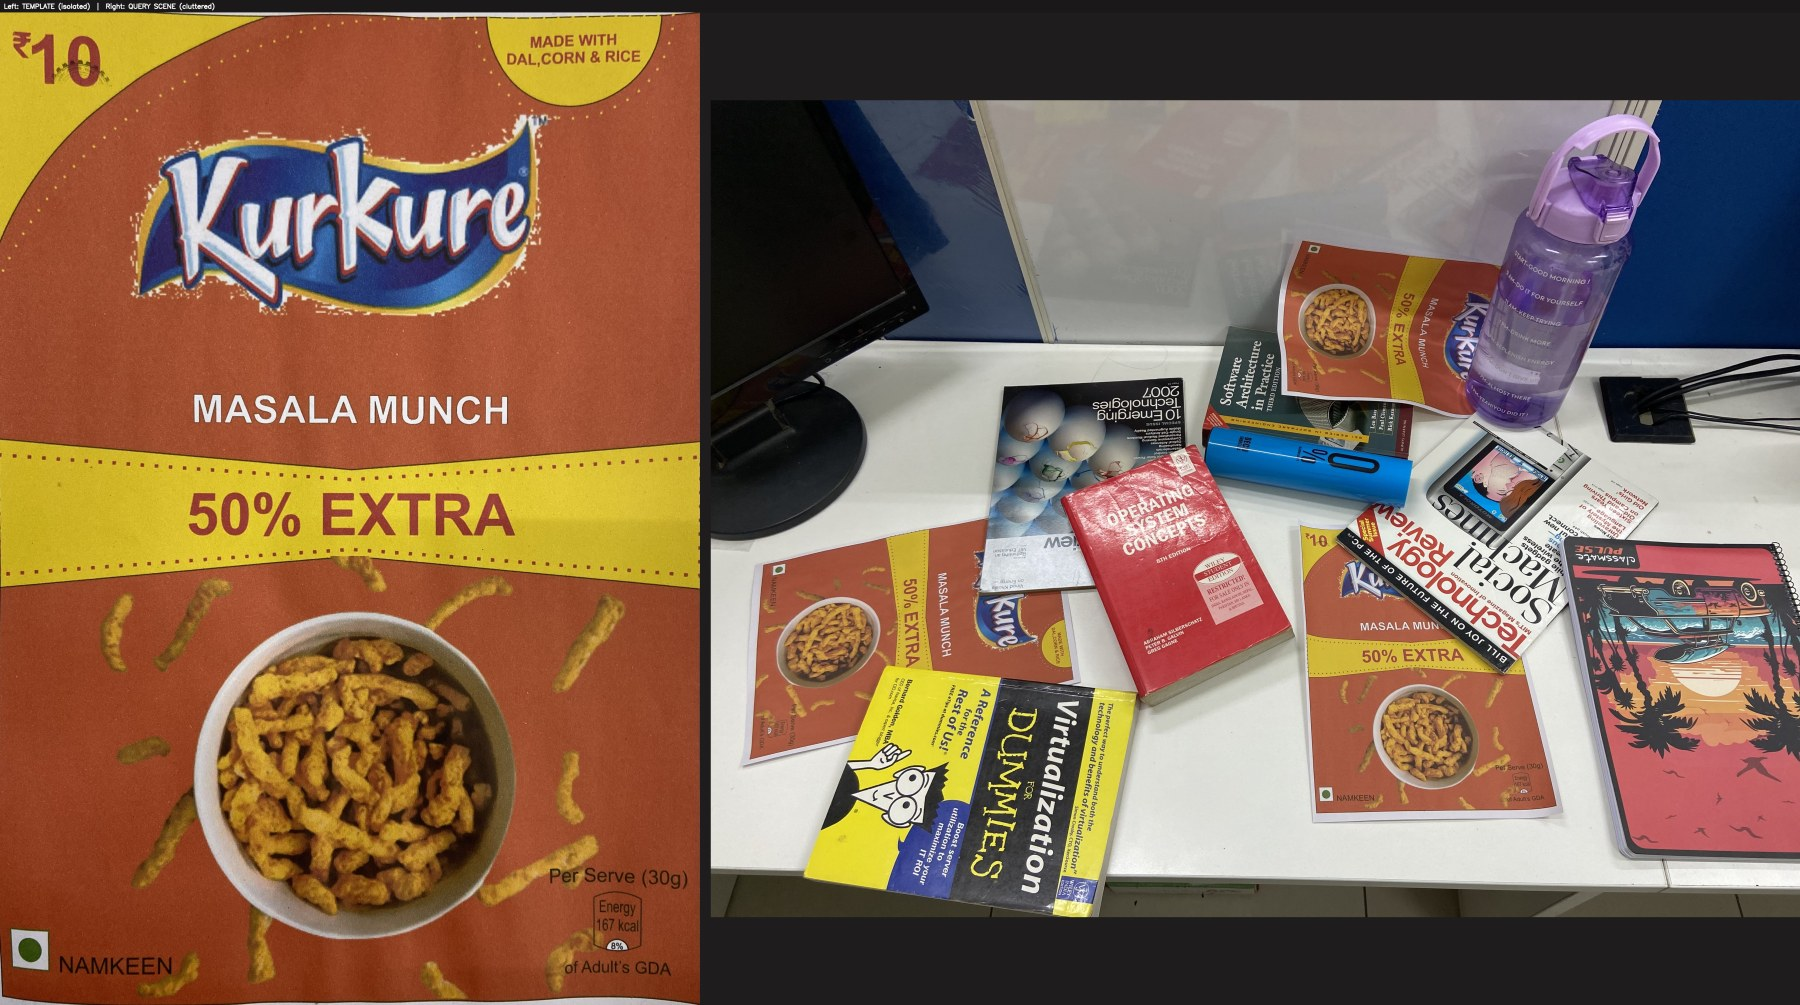
\includegraphics[width=\textwidth]{figs/fig00_inputs.jpg}
\caption{Left: isolated Kurkure template. Right: cluttered lab-desk query.}
\end{figure}

\section{Recognition pipeline}

\subsection{SIFT features}

SIFT keypoints and 128-D descriptors are extracted on both images
(28,667 template keypoints, 38,802 scene keypoints). Descriptors are
$L_1$-normalised and square-rooted (RootSIFT) before matching so that
Euclidean distance corresponds to the Hellinger distance between gradient
histograms.

\subsection{Feature correspondence}

For each scene descriptor the two nearest template descriptors are found by
explicit Euclidean distance. A match is kept only if it passes Lowe's ratio
test
\[
  \frac{d_1}{d_2} < \rho, \qquad \rho = 0.80.
\]
Matching is performed from the scene to the template so that each instance can
accumulate its own correspondences rather than competing for a fixed budget of
template features. This reduced 38,802 nearest-neighbour pairs to 2,842
matches (rejection rate 92.7\%).

\begin{figure}[H]\centering
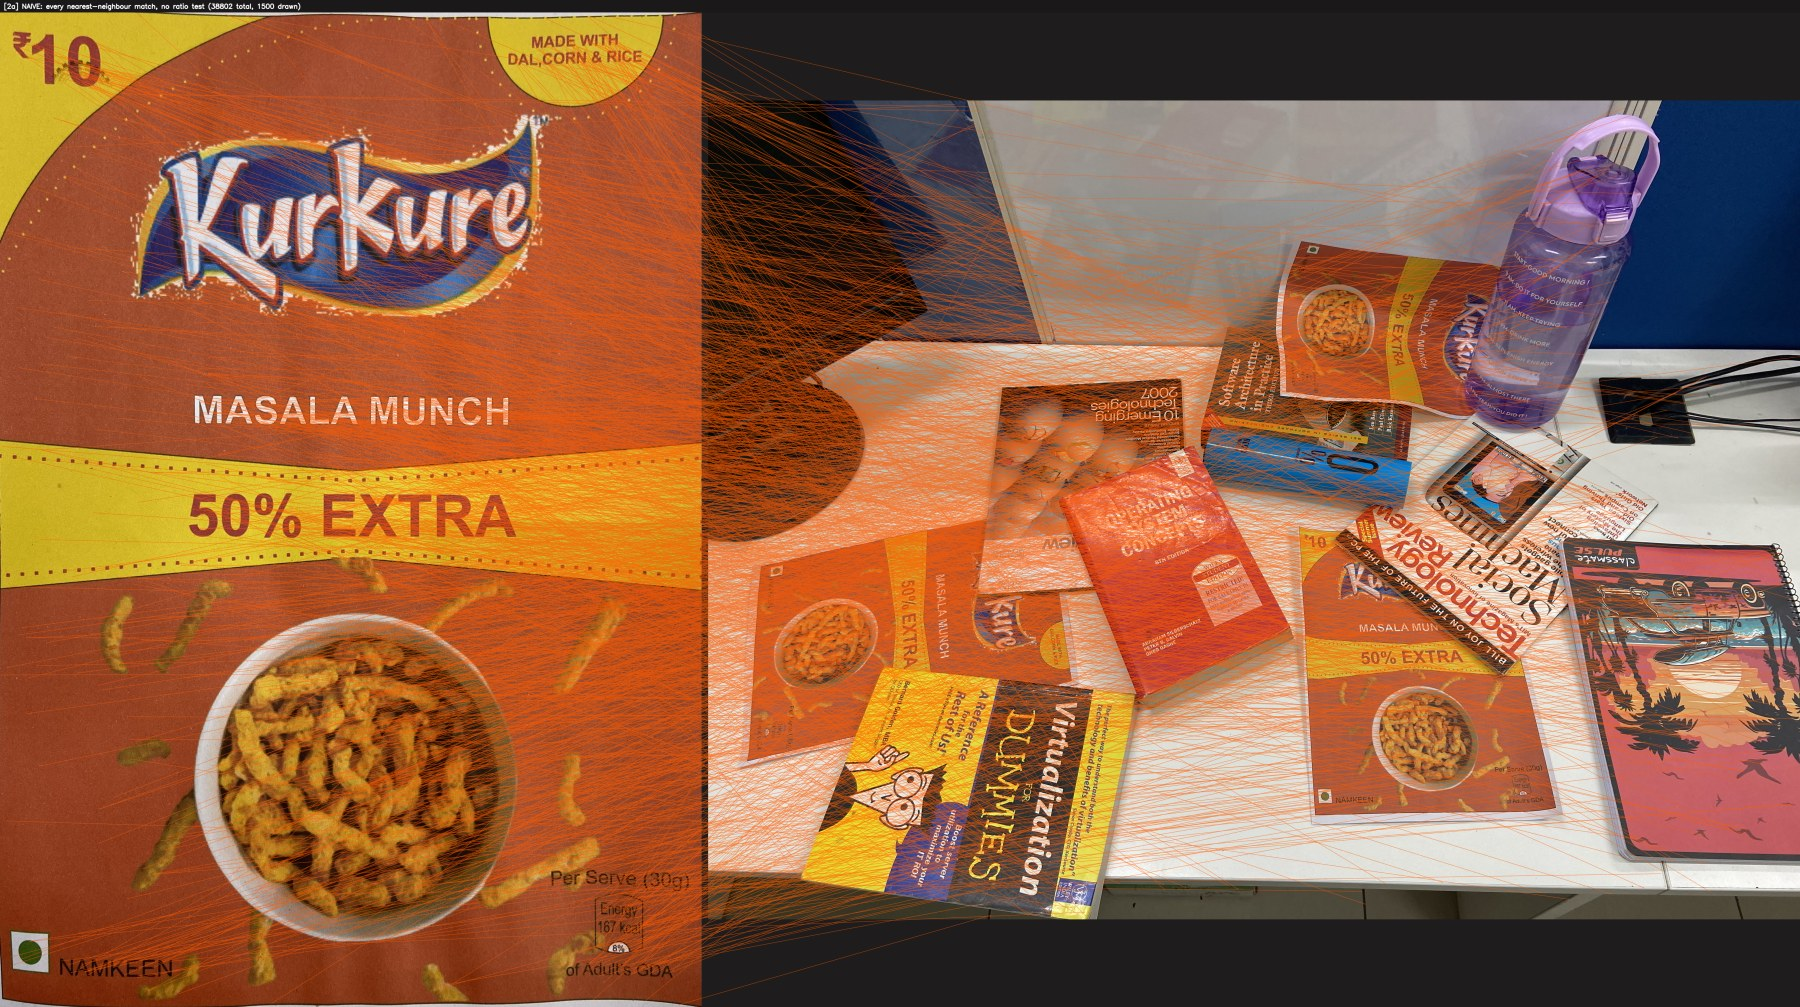
\includegraphics[width=0.96\textwidth]{figs/fig02_naive_all_nn_matches.jpg}
\caption{Naive nearest-neighbour matches without a ratio test. Correspondences
spread across background clutter and do not identify object instances.}
\end{figure}

\begin{figure}[H]\centering
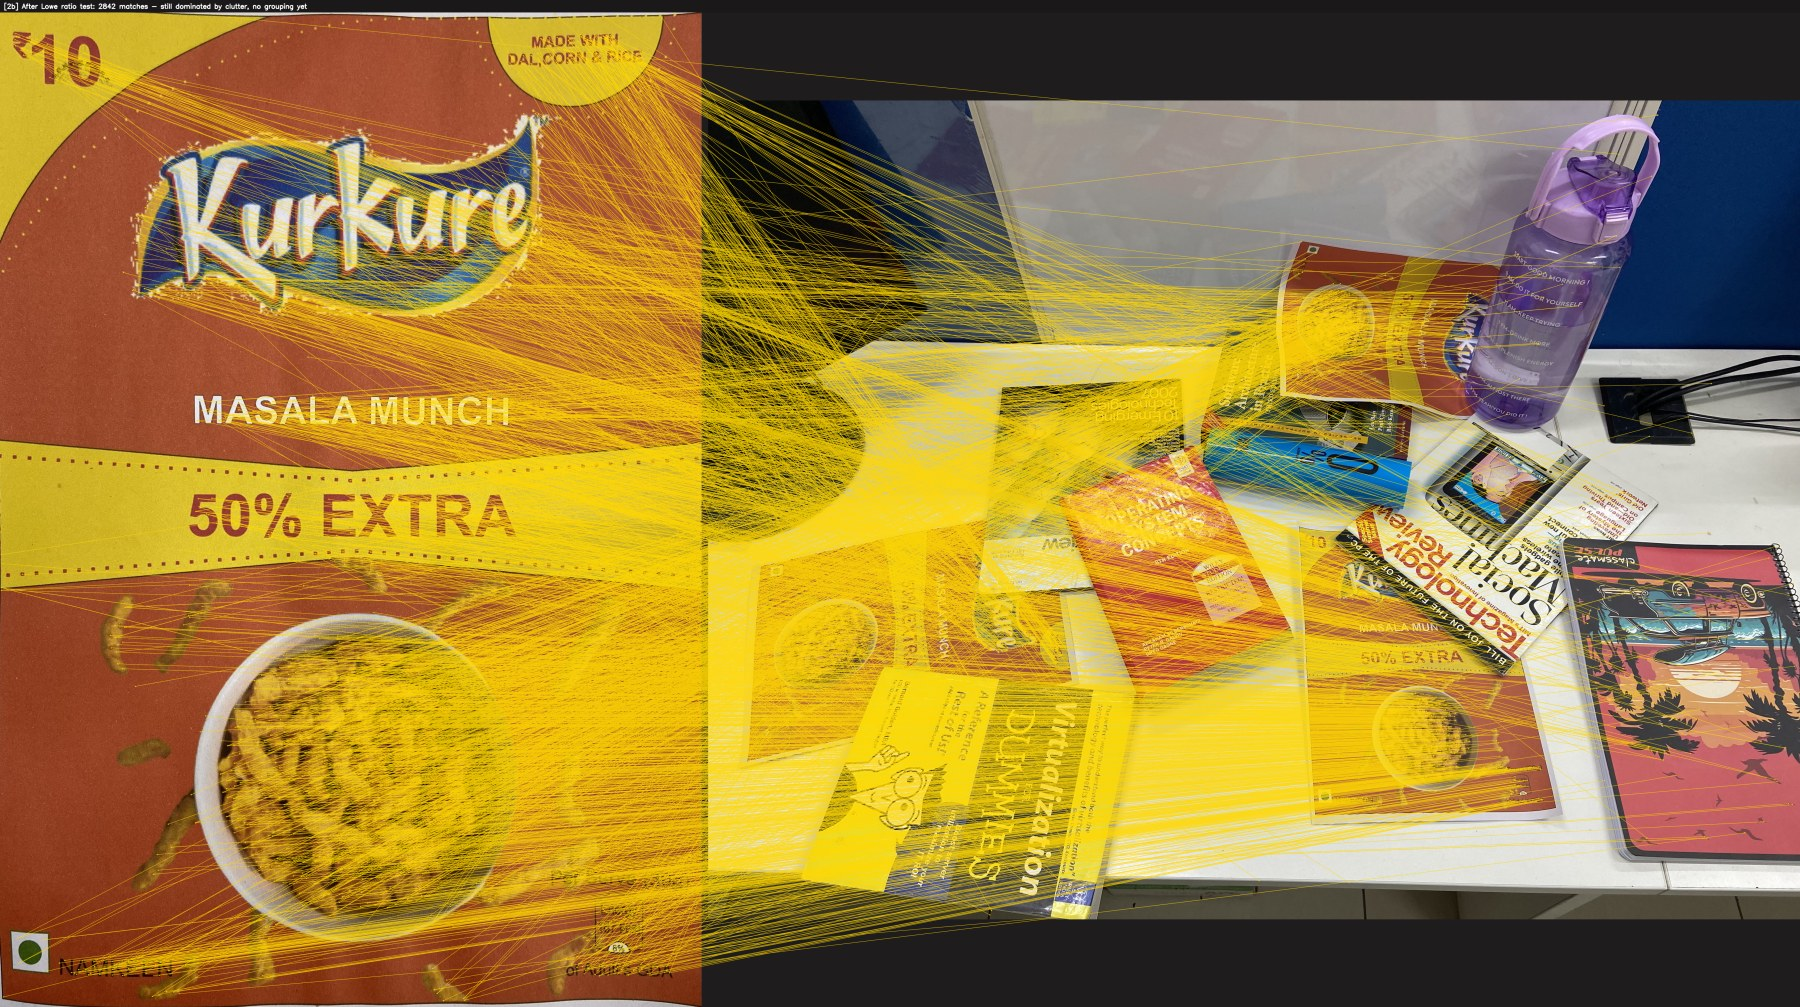
\includegraphics[width=0.96\textwidth]{figs/fig03_after_lowe_ratio.jpg}
\caption{Matches remaining after Lowe's ratio test. Clutter is reduced, but
the output is still an unordered set of correspondences.}
\end{figure}

\subsection{4D generalised Hough transform}

A single SIFT match implies a similarity pose (centre, scale, orientation).
Each match therefore casts a vote in a four-dimensional parameter space
$(c_x, c_y, \log_2 s, \Delta\theta)$. Votes are broadened to neighbouring bins
so that clusters straddling a bin boundary are not split. Bins with at least
three votes form candidate object hypotheses. In this run the vote table
contained 3,037 occupied bins, of which 1,154 cleared the vote threshold; the
strongest bin held 1,031 votes.

\begin{figure}[H]\centering
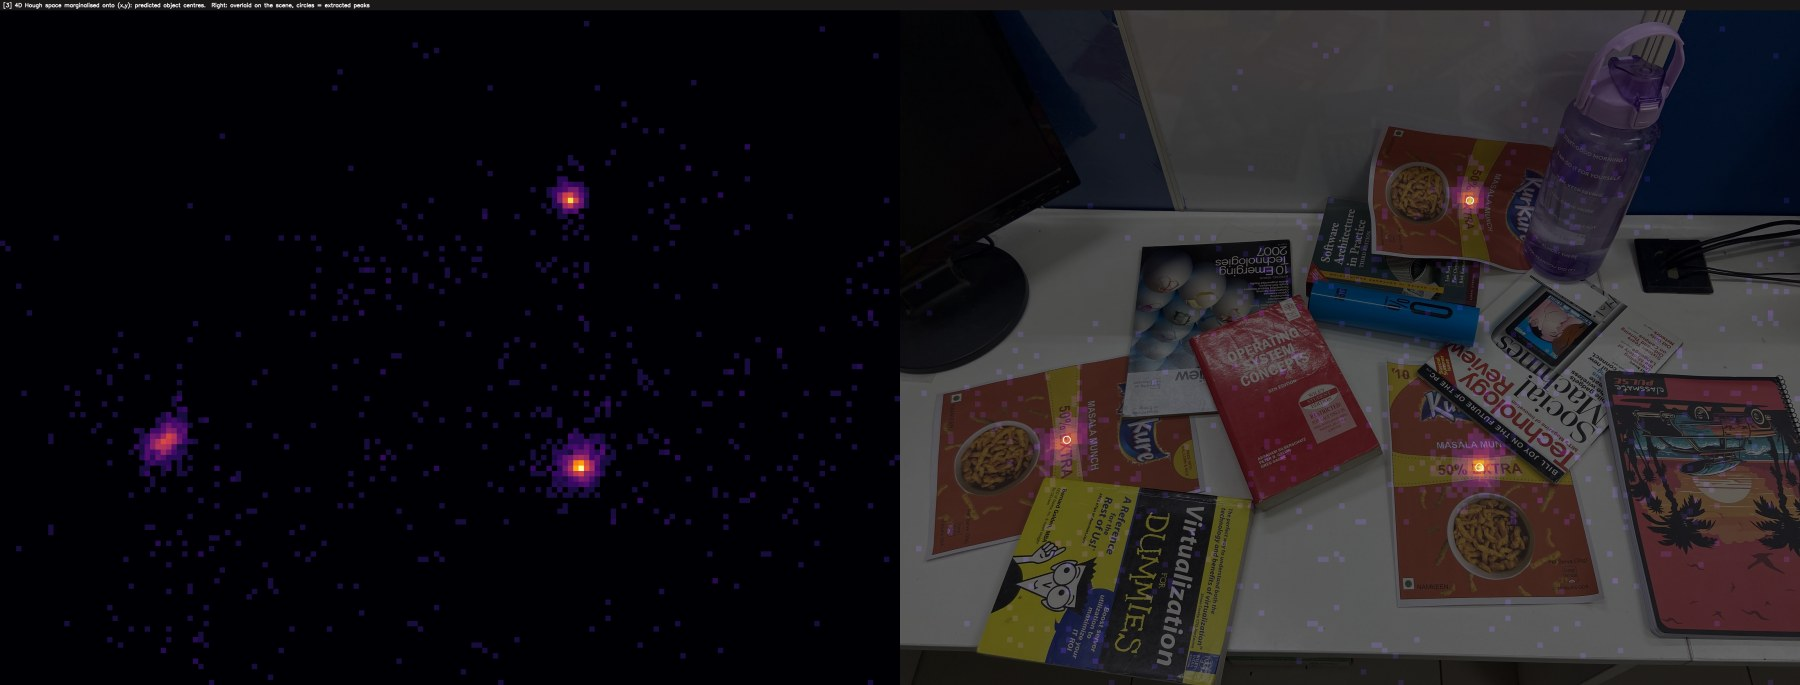
\includegraphics[width=0.96\textwidth]{figs/fig04_hough_vote_space.jpg}
\caption{Hough votes marginalised onto the image plane. Peaks correspond to
likely object centres.}
\end{figure}

\subsection{Robust affine estimation}

For each candidate bin, a 2D affine transform
\[
  \begin{bmatrix}x'\\y'\end{bmatrix}
  =
  \begin{bmatrix}a&b\\c&d\end{bmatrix}
  \begin{bmatrix}x\\y\end{bmatrix}
  +
  \begin{bmatrix}t_x\\t_y\end{bmatrix}
\]
is estimated with RANSAC. Minimal samples of three correspondences are solved
exactly; surviving models are refined by least squares on the inlier set
($A\mathbf{x}=\mathbf{b}$). Degenerate samples are rejected by a collinearity
check, and fitted transforms are discarded if they imply a reflection or
excessive shear.

\subsection{Iterative extraction}

One affine model describes one instance. After a verified detection is emitted,
its inlier matches are removed and the Hough table is rebuilt. The loop repeats
until no remaining bin yields a verified fit. This sequential inlier
subtraction recovers multiple instances without rediscovering the strongest one
repeatedly.

\subsection{Verification and non-maximum suppression}

A hypothesis is accepted only if it has sufficient inliers, a coherent inlier
ratio, acceptable mean reprojection error, geometric sanity, adequate inlier
spread across the template, and a positive appearance check based on zero-mean
normalised cross-correlation. Overlapping boxes that describe the same physical
packet are merged with polygon IoU non-maximum suppression.

\begin{figure}[H]\centering
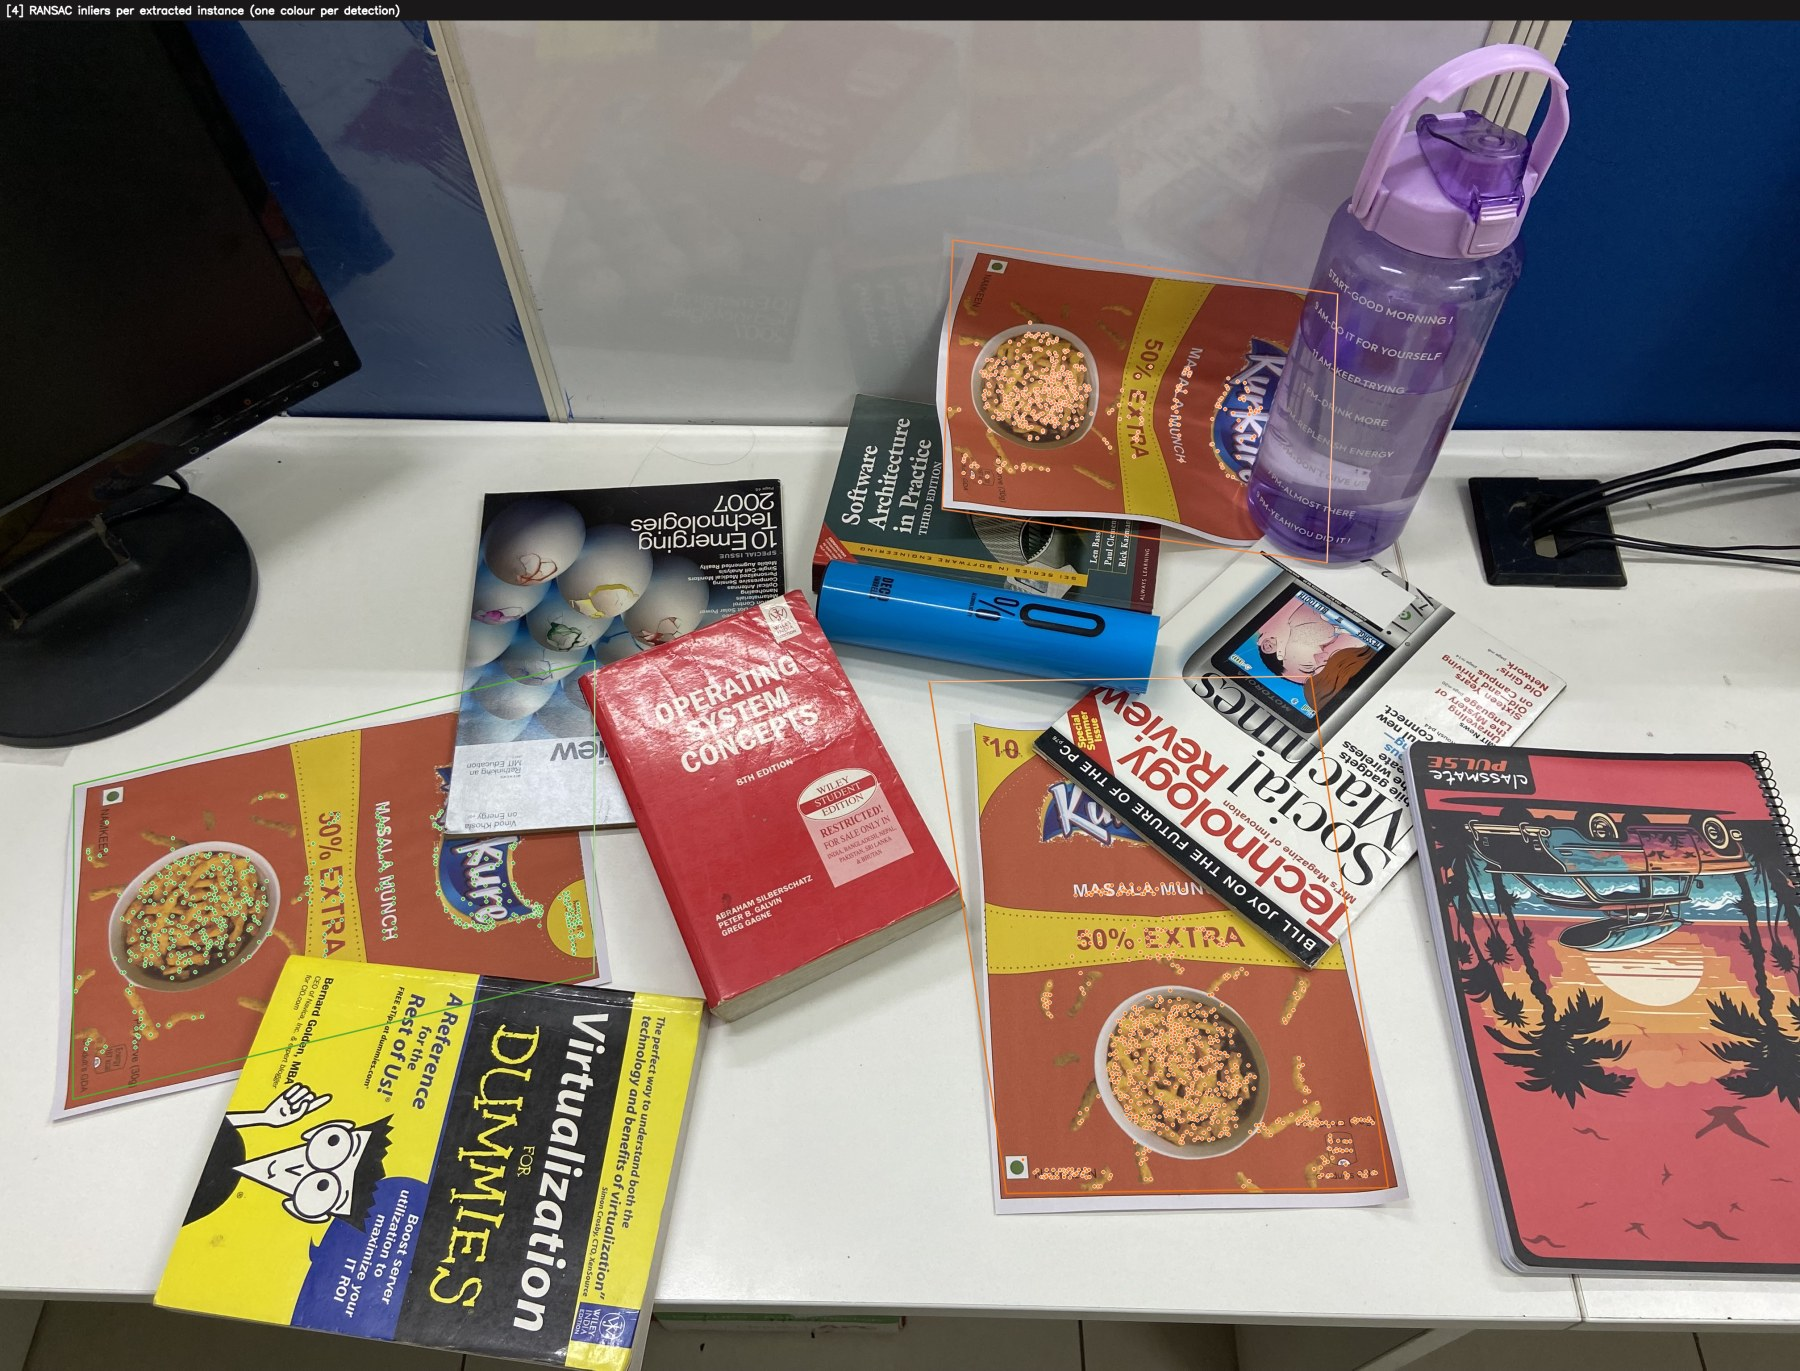
\includegraphics[width=0.96\textwidth]{figs/fig05_inlier_clusters.jpg}
\caption{RANSAC inliers for each accepted instance after greedy extraction.}
\end{figure}

\begin{figure}[H]\centering
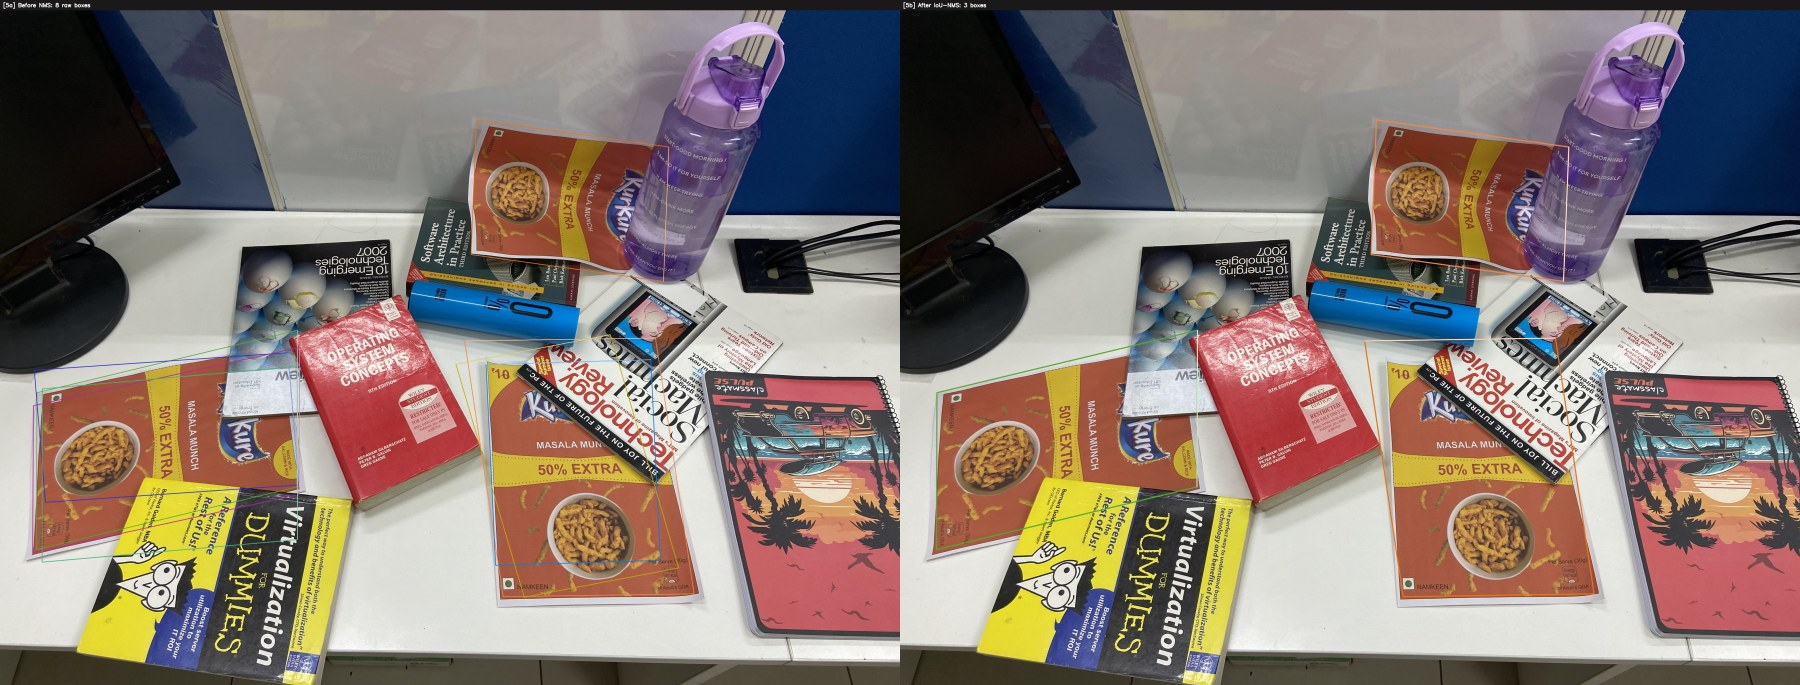
\includegraphics[width=0.96\textwidth]{figs/fig06_nms_before_after.jpg}
\caption{Duplicate suppression: overlapping hypotheses before and after IoU NMS.}
\end{figure}

\section{Results}

The pipeline localised \textbf{3} Kurkure packets on the lab desk.
8 raw hypotheses were produced before NMS; 5 were removed as
duplicates; 295 bins failed verification. Total runtime was 50.0\,s.

\begin{table}[H]\centering\small
\caption{Accepted detections.}
\begin{tabular}{@{}rrrrrrrr@{}}
\toprule
\# & Scale & Rotation ($^\circ$) & Inliers & Inlier ratio & Mean err.\ (px) & ZNCC & $\sigma_{\max}/\sigma_{\min}$ \\
\midrule
    1 & 0.234 & 92.2 & 450 & 0.87 & 6.45 & 0.14 & 1.107 \\
    2 & 0.293 & 90.2 & 594 & 0.92 & 4.81 & 0.39 & 1.358 \\
    3 & 0.321 & 359.1 & 874 & 0.85 & 5.88 & 0.23 & 1.154 \\
\bottomrule
\end{tabular}
\end{table}

\begin{figure}[H]\centering
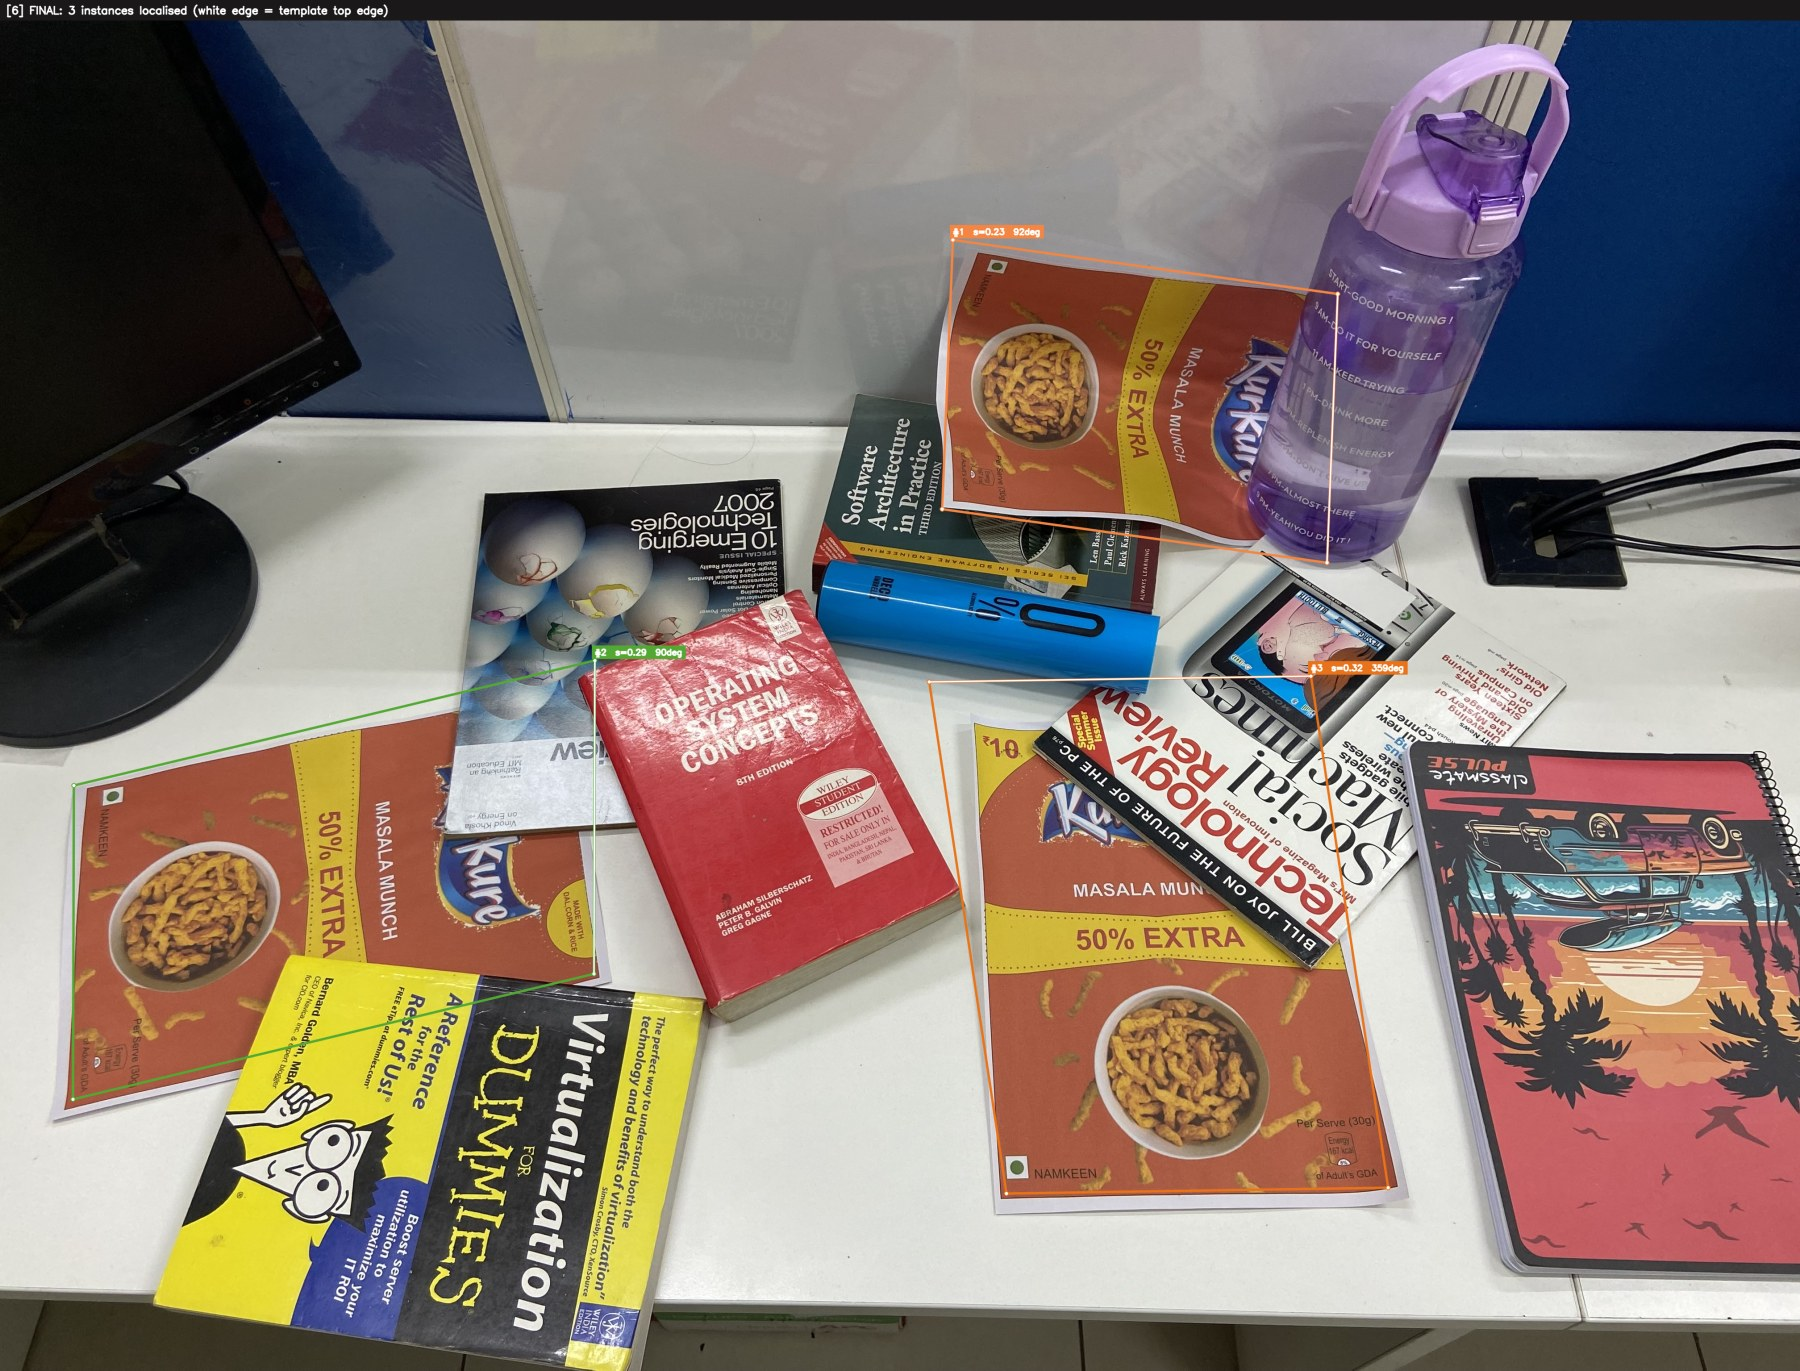
\includegraphics[width=0.96\textwidth]{figs/fig07_final_detections.jpg}
\caption{Final localisations. Each quadrilateral is the template rectangle
projected through the estimated affine transform.}
\end{figure}

\begin{figure}[H]\centering
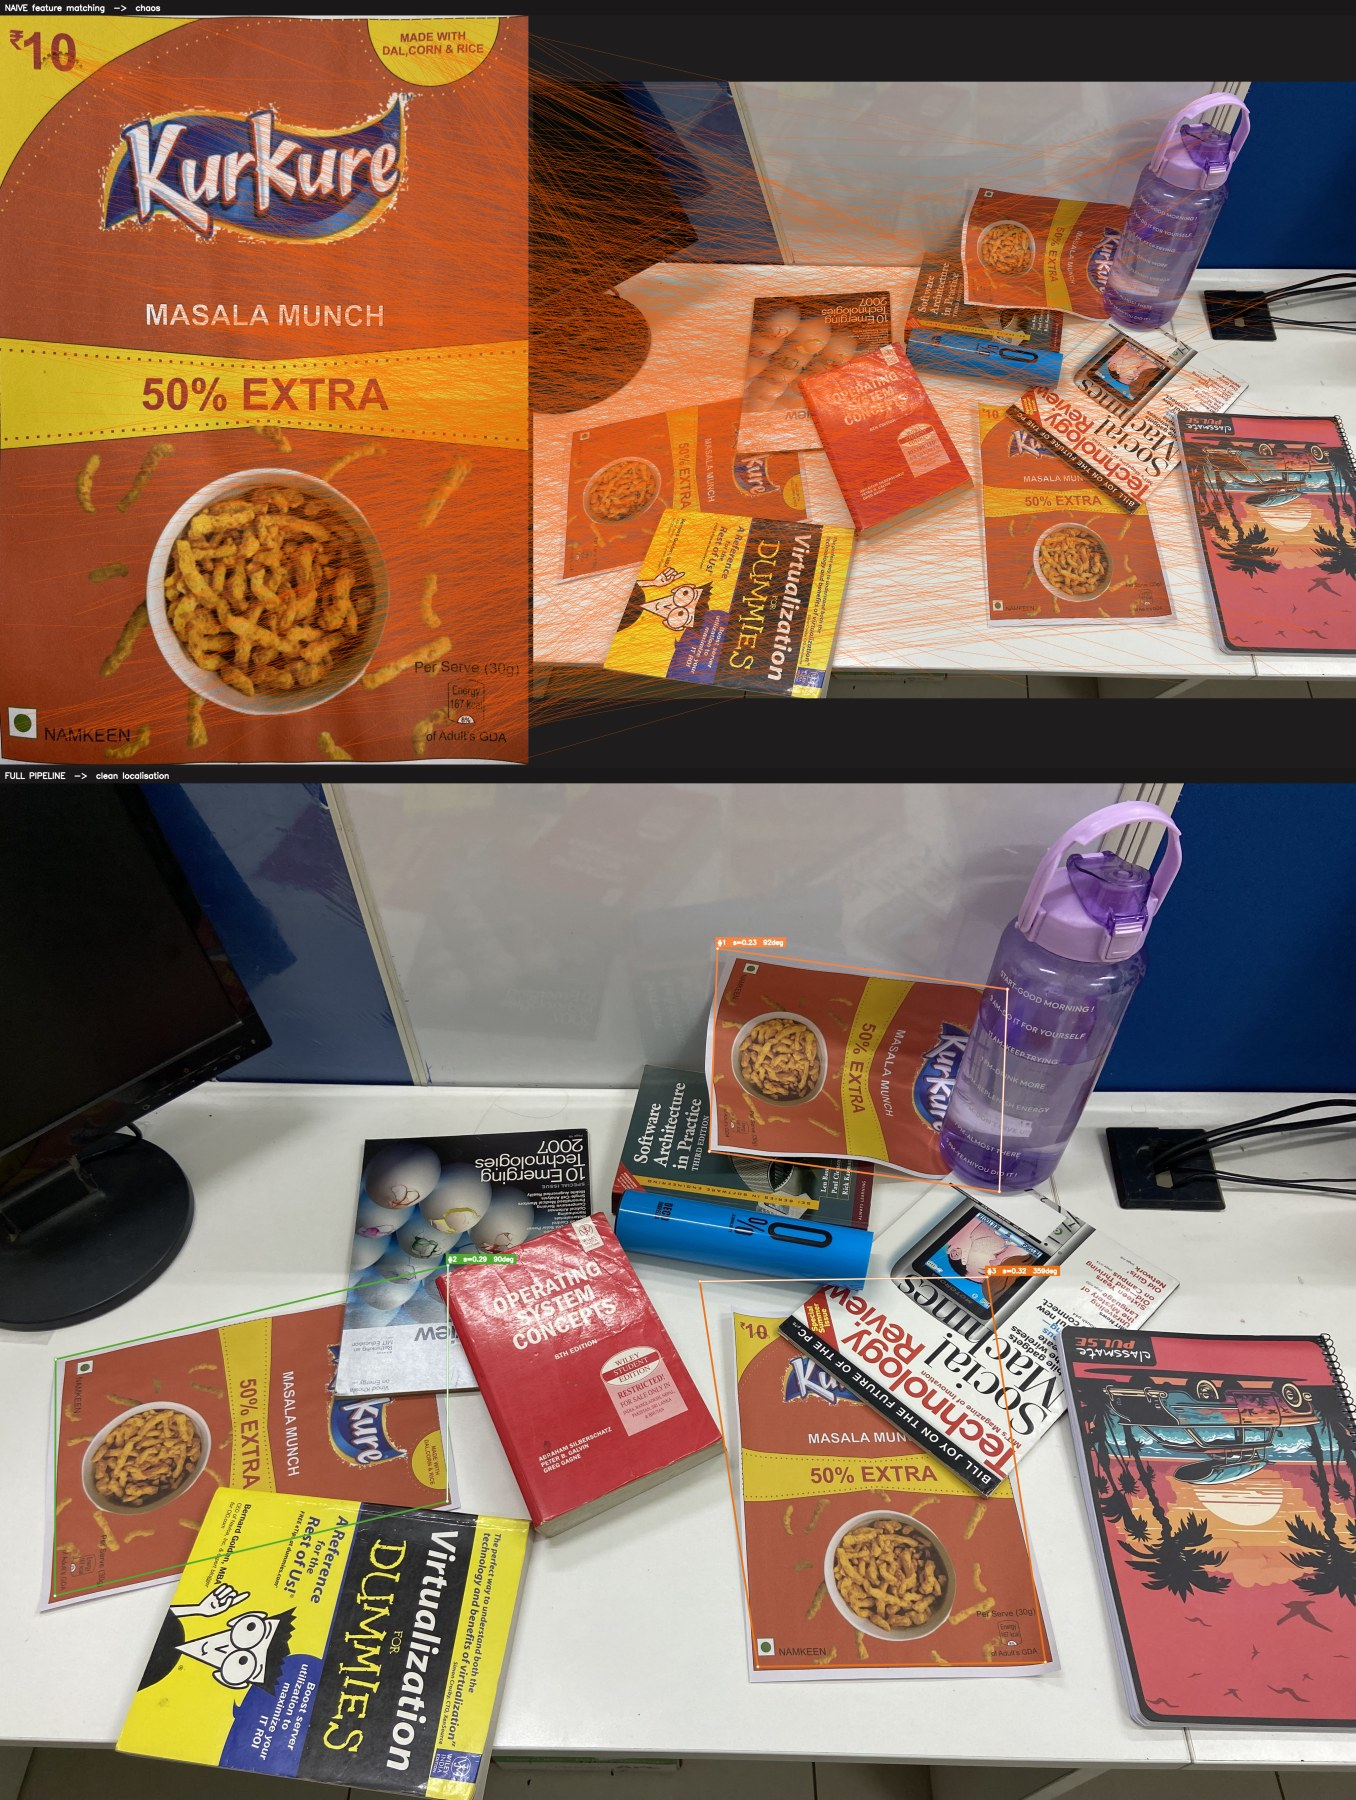
\includegraphics[width=0.92\textwidth]{figs/fig08_comparison_naive_vs_final.jpg}
\caption{Comparison required by the brief: chaotic naive feature matching
versus the final processed bounding-box detections.}
\end{figure}

\section{Discussion}

Naive matching alone is not usable in a cluttered desk scene: most
correspondences attach to background texture. Lowe's ratio test removes a large
fraction of ambiguous pairs, but still leaves an unordered match set. Clustering
in pose space groups those matches into instance hypotheses; RANSAC and the
geometric checks keep the projected boxes from shearing; verification rejects
spurious peaks; and IoU NMS leaves one box per packet.

The recovered scales (about 0.23--0.32 relative to the close-up template) and
rotations near $0^\circ$ and $90^\circ$ match the layout visible in the lab-desk
photograph. Mean reprojection errors on the accepted models are a few pixels on
a 4K scene.

\section{How to reproduce}

\begin{verbatim}
pip install -r requirements.txt
python run_pipeline.py --template data/template.png \
                       --scene data/scene.png --no-gt --out outputs
python make_report.py
\end{verbatim}

\end{document}
